%motivation - representation fairness
In typical blockchain protocols, nodes (such as Bitcoin's miners) have the freedom of choosing which transactions to include in a block. Normally, transactions come along with a fee and nodes choose the highest paying transactions available. In \nameNS, fees do not play a role in $etx$ selection, as they are obfuscated. Instead, there are other factors that lead nodes to prefer certain $etx$s over others. A good example for such a factor can be the identity of the owner node for a certain transaction. The main goal of this section is to introduce to \name a mechanism for selecting $etx$s in a \emph{fair} manner. Fairness in this regard should be reflected by the blockchain, representing each node according to the portion of $etx$s it owns\footnote{In future work we will refer to some problems that such fairness may yield, e.g., that nodes artificially produce many self-owned transactions in order to get more block real-estate.}. %In a nutshell, this is solved by a fee mechanism.}.

An important aspect in the context of fair sampling in \nameNS, is the relation between the rate at which $etx$s are issued and the rate at which they are appended to the blockchain. An epoch at which the \emph{issuance rate} is smaller than the maximal \emph{append rate} allowed by the system  is relatively easy to analyze - all transactions are processed within a small time frame. A more involved case is when the issuance rate is (temporarily) greater than the append rate. During such epochs, there are many $etx$s pending to be added to the blockchain. This makes the decision of which $etx$s to include in an Eblock more significant and subject to manipulations, which is something we wish to limit. We thus assume throughout this section that the size of a correct node's Epool is greater than $b$ (the maximal number of $etx$s in an Eblock). %This implies that \emph{the size of a proposed Eblock is exactly $b$}. 

To achieve \emph{representation fairness}, we adapt a strategy of correlated sampling of a single element to a method that samples many elements. We use this sampling procedure for choosing transactions from one's Epool in a way that emulates random selection. Furthermore, this procedure is \emph{verifiable} in the sense that a node validating a proposed Eblock, can check that the $etx$s it contains were selected legally. This ensures that Byzantine primaries cannot exploit high-load epochs to their benefit by over-servicing favored nodes.

Correlated sampling, considered in~\cite{HashSample1},~\cite{HashSample2},~\cite{HashSample3} (see 
also~\cite{OptCorSampling} for a review and optimality result) refers to the problem in which there are two players having different distributions over the same domain (in our case the global Epool) and access to shared randomness (in our case the random seed). The two players wish to output a single element each sampled according to their distributions while minimizing the probability that their outputs differ. 
In the work of~\cite{HashSample1} a MinHash strategy was used for performing correlated sampling for the case that the distributions are uniform over a subset of the domain. In~\cite{hashsamplemultiple} Rivest applied the MinHash strategy sequentially in order to sample many elements from the domain, possibly with repetitions. However, to the best of our knowledge the question of correlated sampling of many elements \textbf{without} repetitions was not considered before.   

%Section structure
In this section we describe the procedure for selecting $etx$s and the way nodes validate them in \nameNS. Then, we analyze the benefits and risks introduced to the protocol by these modifications, in terms of liveness and fairness of the protocol.
We refer to term number $r$ and explain the construction and validation process of $EB^r$.

\subsection{Eblock construction and validation}
Our correlated scheme uses a hash function in order to serialize candidate $etx$s for the next Eblock. The hash function is initialized with a random seed to eliminate its predictability, yielding a common, random and unpredictable serialization of the $etx$s. Primaries are asked to include in $EB_p$ their $b$ lowest hashed $etx$s. Committee members are asked to validate this selection by comparing $EB_p$ with the lowest hashed $etx$s of their own Epools. $EB_p$ is validated iff the intersection of these two sets is large enough for enough committee members. 

The validation conditions are set such that eventhough different Epools differ slightly due to network latency, correct nodes accept validly constructed Eblocks with overwhelming probability. If, on the other hand, the primary chooses to include in $EB_po$ $etx$s which are not among its $b$ lowest, (in order to over service its own users), then $EB_p$ has a lower probability of passing validation and is more likely to get rejected. 

\textbf{Eblock Construction}. We start with the notion of a node \emph{locking} its Epool. We denote by $EP_i^t$ node $i$'s locked Epool at time $t$, which is a snapshot of the $etx$s in $i$'s Epool at time $t$\footnote{This can be implemented by attaching a timestamp to each $etx$ at the time it was received.}. We denote by $t_i$ the time at which node $i$ received $DB^{r-1}$, the Decrypted-block at term $r-1$, and define the \textit{locking time} of node $i$ to be $t_i-2\Delta$. The idea behind the locking time will be clarified shortly.

The primary node $p$ constructs its Eblock, denoted $EB_p$, by choosing the $b$ $etx$s in $EP_p^{t_p-2\Delta}$ that hash to the minimal values according to $H(RS^{r-1},etx)$. We note that $RS^{r-1}$, which was already used to randomly select the committee members in term $r$, is used here again as a random and unpredictable seed for the hash function. 

The choice of a locking time is done in order to ensure that network latency does not allow a quick node to prepare and forward tailor-made $etx$s (in terms of their hash values), \emph{after} revealing the random seed, but \emph{before} the rest of the network does.  
Due to network latency, it could be the case that $RS^{r-1}$ is revealed to some node before the rest of the network - by at most $2\Delta$ time. It can exploit this extra time to generate $etx$s with low hash value (i.e., with low $H(RS^{r-1},etx)$) and disseminate them to the network. Restricting the nodes to consider only $etx$s which were known to them prior to time $t_i-2\Delta$ prevents this kind of attack. 
% A more elaborate explanation to this claim can be found in \ref{subsec:repfair}.

%We note that not only the primary constructs an Eblock in term $r$. 
In addition to the primary node, all correct committee members construct a local version Eblock, $EB_i$, which includes the $b$ $etx$s with lowest hash value among all $etx$s in $EP_i^{t_i-2\Delta}$. $EB_i$ is compared to $EB_p$ as part of the validation process. 

%notations: $EB_i$
%validating an Eblock in term $r$
\textbf{Eblock Validation}. Upon receiving a proposal of an Eblock $EB_p$ from the primary, a correct committee member $i$ validates it by performing the validation process presented in~\ref{Protocol:ValidateEB}, along with two additional steps: 
\begin{enumerate}
\item There are exactly $b$ $etx$s in $EB_p$.
\item $ |EB_p\cap EB_i|\geq  \beta(b) \cdot b$. That is, there is at least a $\beta$-fraction overlap between the $etx$s in the Eblock $i$ constructed and that of the primary. The parameter $\beta$ depends on how large the overlap between two different correct nodes' Epools is and on the size of the Eblock $b$.
% $$$$$$$\item TODO: add an additional condition - threshold $$$$$$$
\end{enumerate}


%Explanation as to the locking times choices
%\red{VERSION 1:}

%Locking a validating committee member's Epool at $t_i-2\Delta$ ensures that the primary could not have the time to dissipate tailor-made $etx$s for term $r$. Due to the synchrony assumptions we have, it is guaranteed that the primary could not have revealed $DB^{r-1}$ (and thus also $RS^{r-1}$) prior to $t_i-2\Delta$. Put differently, $t_i-2\Delta < t_p$ (recall the decryption process). 

%Explanation as to why $\alpha$ can be assumed close to $1$
%To maintain the liveness of the protocol, we rely on a large overlap between their Epools at the locking time, that is between $EP_p^{t_p-2\Delta}$ and $EP_i^{t_i-2\Delta}$. The locking time of the validators is enforced upon us to ensure no tailor-made $etx$s are dissipated. The locking time of the primary, on the other hand, is chosen to maximize its overlap with the other Epools (at their locking time), so as to increase its chances of being validated. In absence of any other information, the primary's best guess is that $t_i\sim t_p$, that is, the decryption time of the primary is roughly the same as the other node's decryption time. In this way, it is safe to assume that at the locking time, the primary's Epool is similar to other nodes' Epools. 

%Justification: the deterministic rule emulates a random sample of one's Epool.
%Thus far we have argued that the deterministic $etx$ selection procedure emulates a random sample of one's Epool. We showed that no primary can manipulate nodes' Epools after revealing $RS^{r-1}$ by quickly forwarding low-hashed $etx$s for term $r$. Following similar logic, it is also true that other nodes cannot manipulate the primary's Epool and have it construct an Eblock with a disproportionate amount of their $etx$s.

%What are the risks introduced by these modifications?
%In the following section we show that the deterministic selection procedure and the validation process that goes with it maintains Gruffalo's basic properties: 
%\begin{itemize}
%\item Safety. We are only limiting the valid Eblocks and thus safety is not affected.
%\item election-fairness. We did not change the way $RS^r$ is being produced and thus this property is kept trivially.
%\item Liveness (strong liveness). We show later that with overwhelming probability a validly constructed Eblock gets committed.
%\end{itemize}

%What do we gain from this?
%representation fairness
%We then show the main gain to Gruffalo from this modification, namely that Gruffalo is \emph{$\epsilon$-representation fair} (as defined later). This is a consequence of the fact that with this validation method, the power of a Byzantine primary to construct an unfair Eblock is limited. 


%Explanation as to the locking times choices
\textbf{Tradeoff in the selection of $\pmb{\beta}$}: Setting the parameter $\beta (b) \in [0,1]$ (as a function of the block size $b$) is a critical task. On the one hand, a larger $\beta$ guarantees solid \emph{representation fairness}, which is simply to say that nodes' representation in Eblocks is similar to their relative $etx$s issuance rate. On the other hand, the larger $\beta$ is, committee members are more strict in validating Eblocks. Thus, potential differences between Epools of correct nodes might result in Eblocks being often rejected, and guaranteeing liveness becomes more difficult. %\red{further explanation needed, I would rephrase}. 

In the next section we find an appropriate $\beta$, that does not risk the liveness of the protocol. Then, we show to what extent is the protocol representation fair with respect to that $\beta$.

%Explanation as to why $\alpha$ can be assumed close to $1$

%Justification: the deterministic rule emulates well random sampling of one's Epool. A proposed Eblock will be validated against an Epool prior to the time the primary could have constructed the Eblock.

%intuition as to each added step in the validation process

%validating $th^r$ assuming close Epools at any point in time for any correct pair.

%validating the content of an Eblock.


%Intuition as to each new step

%What do we gain from this?
%representation fairness
%What are the risks introduced by these modifications?

%Question:
%Can we check that a proposed Eblock is only contained within the validating Eblock? or do we have to look at the intersection? I ask because we can verify a correct primary constructs its Eblock according to an older Epool and thus at the construction time an $etx$ selected by the primary is with high probability known to the validators. Vice versa though, is not true...
%This is a softer condition than the intersection - thus it shouldn't affect liveness. What about representation fairness?

\subsection{Liveness in High-load epochs} \label{Liveness}
%The problem in Gruffalo's terms
	%(Repetitive) The main goal of the validation condition is to restrict the primary's ability to deviate from a random selection of $etx$s, which would ensure \textit{representation fairness}. 
To maintain \emph{strong liveness}, we must guarantee that an honestly constructed Eblock gets committed w.o.p.. It is enough to show that a correct committee member accepts a proposed Eblock as long as it was constructed according to the correlated sampling procedure. This is achieved if $\beta$ is properly chosen.

A careful choice of $\beta$ would take into account the extent to which Epools can differ at locking time. Due to network latency and inherent properties of the protocol, we cannot expect $EP_i^{t_i-2\Delta}$ and $EP_j^{t_j-2\Delta}$ to be identical. To model this difference we consider the set $GEP^t$, which is the \emph{global Epool} at time $t$ satisfying $GEP^t = \cup_{i}EP_i^t$. It contains all issued $etx$s not yet appended to the blockchain by time $t$. 
%We have $EP_i^t\subseteq GEP^t$ for any correct node $i$ and time $t$. 

%Define $t^r:=max_i\{t_i-2\Delta\}$ \red{($i$ should be correct, why $r$? Maybe it can be rephrased: "denote by $t^r$ the maximal locking time of a correct node (in term $r$), let $t^r$ be the locking time of $GEP$".)} 

Denote by $t^G$ the maximal locking time of a correct node $t^G = max_i\{t_i-2\Delta\}$. We refer to $t^G$ as the locking time of $GEP$, and refer to $GEP^{t^G}$ as $GEP$. Notice that the locking times of two nodes are slightly different (even those of two correct nodes). Moreover, network latency in general results in a slight difference between two Epools - even when both are considered at the same time $t$. For these reasons, we cannot expect to have $EP_i^{t_i-2\Delta}=EP_j^{t_j-2\Delta}$. However, as locking times are similar, and network latency not too significant, we do assume a measure of (at least) $\alpha$-fraction similarity bound between $EP_i^{t_i-2\Delta}$ and $GEP^{t^G}$ for any correct node $i$. Precisely, for a correct node $i$, we have $|EP_i^{t_i-2\Delta}| \geq \alpha|GEP|$.
From this we can induce a simple probabilistic model which states as follows: $EP_i^{t_i-2\Delta}$ is a random sample of $GEP$, where each $etx\in GEP^{t^G}$ is included in $EP_i$ with probability at least $\alpha$.

\begin{claim} [liveness under correlated sampling] Let $\beta(b) = \alpha^2 - \sqrt{\frac{10}{b}}$. For two correct nodes $p$ and $i$, $i$ accepts $p$'s proposed Eblock $EB_p$ w.o.p., i.e., $|EB_p\cap EB_i|\geq \beta \cdot b$ holds w.o.p.. 
\end{claim}

\red{We make the important observation that in the real world network, the exact value of $\alpha$ is not known to any node. In order to still use it in our algorithm, $\alpha$ would have to be set as a parameter of the protocol, which is agreed upon among all nodes, and that would serve as a lower bound on the similarity between any two correct nodes.}



\begin{proof}
Let $GEB$ be the set of $b$ $etx$s in $GEP$ with lowest hash values (i.e., the $b$ lowest $H(RS^{r-1},etx)$). We define $Y_{etx}$ to be the indicator random variable stating whether $etx\in EP_p\cap EP_i$, namely 
\begin{equation}
    		Y_{etx} =	
		    \begin{cases}
    			  1  &\mbox{if }  etx\in EP_p\cap EP_i \\
     			  0  &\mbox{otherwise}
		     \end{cases}.
  	\end{equation} 
Notice two things: First, these random variables are i.i.d. Bernoulli variables, with success probability of at least $\alpha^2$. Second, for any correct node $j$ and an $etx \in EP_j$, if $H(RS^{r-1},etx)$ is among the lowest $b$ values among the $etx$s in $GEP$, it must be among the lowest $b$ values in $EP_j$. Put differently, $etx\in GEB\cap EP_j \Rightarrow etx\in EB_j$. Define $Y=\sum_{etx\in GEB} Y_{etx}$, and note that $Y\leq |EB_p\cap EB_i|$ (this is in general an inequality since $EB_p$ and $EB_i$ may share $etx$s which are not in $GEB$). Using Hoeffding's inequality, we get
$$Pr \left( \frac{1}{b}|Y-\mathbb{E}(Y)| >\delta \right) \leq exp(-2b\delta^2).$$

Consider an overwhelming probability of at least $1-exp(-20)$. 
Bounding the above probability by $exp(-20)$, we derive an inequality $2b\delta^2 \ge 20\iff \delta \ge \sqrt{\frac{10}{b}}$. 
Trivially, the expected value of $Y$ is lower bounded by $\alpha^2 b$. 
Taking $\delta=\sqrt{\frac{10}{b}}$ and plugging this into the left-hand side of the equation above, we get that w.o.p.  
\begin{equation}\begin{split}|EB_p\cap EB_i|\geq Y&>\mathbb{E}(Y)-b\delta\\ &\ge \alpha^2\cdot b -\sqrt{10b}\\
&=\left( \alpha^2-\sqrt{\frac{10}{b}} \right) b\end{split}\end{equation}
as claimed.
\end{proof}
%Proof of claim (formal)

The claim establishes the fact that w.o.p. \name is strongly live (as formalized in Definition~\ref{definition_strong_liveness}).
In the next section we show how the Eblock construction method results in \name being representation fair.
While the used value of $\beta = \alpha^2-\sqrt{\frac{10}{b}}$ is a function of the similarity bound $\alpha$ and the block size $b$, a lower bound on the value of $\beta$ holds in practical settings.
%b = 200 or 2000 ??
For $\alpha \ge 0.95$ and $b \ge 2000$ it satisfies $\beta \ge 0.83$. 
Table~\ref{tab:table1} illustrates the values of $\beta$ for $\alpha \in \{0.90,0.95\}, b \in \{1000,2000,5000\}$. Values of $\beta$ are also presented 
in Fig.~\ref{fig:beta_vs_alpha}.  
 
% For the definitions and proofs of the next section, it would be much more convenient to think of $\beta\cdot b$ as a linear function of $b$, rather than the current bound which involves a $\sqrt{b}$ factor. For this purpose, we can consider one of the configurations for $\alpha$, $b$, $\delta$, $\beta$ suggested in the table below: 

\begin{table}[h!]
  \begin{center}
    \caption{$\beta$ calculated for different values of $\alpha$ and $b$}
    \label{tab:table1}
    \begin{tabular}{c|c|c|c} % <-- Alignments: 1st column left, 2nd middle and 3rd right, with vertical lines in between
      $b$ & $\alpha$ &$\alpha ^2$ &  $\beta$ \\
      \hline
      1000&0.90 &0.8100&0.7100\\
      1000&0.95 &0.9025&0.8025\\
      2000&0.90 & 0.8100 & 0.7393\\
      2000&0.95 &0.9025&0.8317\\
      5000&0.90 & 0.8100 & 0.7653\\
      5000&0.95 &0.9025&0.8578\\
    \end{tabular}
  \end{center}
\end{table}


\begin{figure}[!t]%[!ht]
\centering
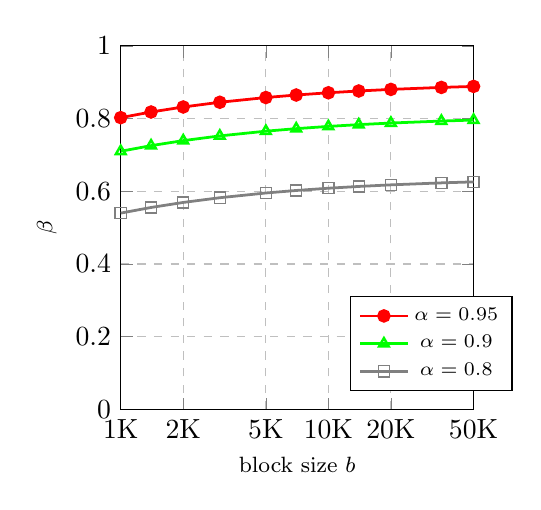
\begin{tikzpicture}
\begin{axis}[
xmode=log,
   xlabel={block size $b$},
   ylabel={$\beta$},
    %ylabel={$\phi(x)$},
    xmin=1000, xmax=50000,
    ymin=0, ymax=1,
    xtick={1000, 2000, 5000, 10000, 20000,50000},
    xticklabels={1K, 2K, 5K, 10K, 20K,50K},
    ytick={0,0.2,0.4,0.6,0.8,1},
    legend pos=north west,
    ymajorgrids=true,
    grid style=dashed,
    height = 6.2cm,
    width = 0.50*\textwidth,
 %   line width=1.6pt,
%]
                legend style={at={(0.65,0.05)},anchor=south west,font=\scriptsize},
                label style={font=\footnotesize}, grid=both];
            %\addplot [black,mark=x] table [x={chi}, y={cooperative}] {\resfirsta};
        \addplot[% only marks, mark=square,  black,mark=
   color=red,mark=*,scale=10, line width=1pt,mark options={line width=0.9pt,draw=red,fill=red}]
    coordinates {
(1000, 0.8025) (1400, 0.8179845745271483) (2000, 0.8317893218813452) (3000, 0.8447649730810374) (5000, 0.8577786404500042) (7000, 0.8647035526990773)(10000, 0.8708772233983162) (14000, 0.8757738758087575) (20000, 0.8801393202250021) (35000, 0.8855969149054297) (50000, 0.8883578643762691)
    };
    \addlegendentry{$\alpha = 0.95$};
    \addplot[% only marks, mark=square,  black,mark=
   color=green,mark=triangle,%dotted, 
   scale=10, line width=1pt,mark options={line width=0.9pt,draw=green,fill=green}]
    coordinates {
        (1000, 0.7100000000000001) (1400, 0.7254845745271484) (2000, 0.7392893218813453) (3000, 0.7522649730810375) (5000, 0.7652786404500043) (7000, 0.7722035526990774) (10000, 0.7783772233983163) (14000, 0.7832738758087576) (20000, 0.7876393202250022) (35000, 0.7930969149054298) (50000, 0.7958578643762692)
    };
    \addlegendentry{$\alpha = 0.9$};
\addplot[% only marks, mark=square,
   color=gray,mark=square,scale=10, line width=1pt,mark options={line width=0.5pt,draw=gray,fill=gray}]
    coordinates {
   (1000, 0.5400000000000001) (1400, 0.5554845745271485) (2000, 0.5692893218813454) (3000, 0.5822649730810375) (5000, 0.5952786404500043) (7000, 0.6022035526990774) (10000, 0.6083772233983163) (14000, 0.6132738758087577) (20000, 0.6176393202250022) (35000, 0.6230969149054298) (50000, 0.6258578643762692)
    };
    \addlegendentry{$\alpha = 0.8$};
\end{axis}
\end{tikzpicture}
\caption{The value of $\beta$ calculated for different values of $\alpha$ and $b$}
\label{fig:beta_vs_alpha}
\end{figure}

% The claim establishes the fact that Gruffalo is strongly live. In the next section we show how the Eblock construction method results in Gruffalo being representation fair. For the definitions and proofs of the next section, it would be much more convenient to think of $\beta\cdot b$ as a linear function of $b$, rather than the current bound which involves a $\sqrt{b}$ factor. For this purpose, observe that $\sqrt{10b}\leq\epsilon b\iff \sqrt{\frac{10}{b}}\leq \epsilon$, and conclude that for any (fixed) $\epsilon>\sqrt{\frac{10}{b}}$, we have $|EB_i\cap EB_p|>\beta b$ for $\beta=\alpha^2-\epsilon$.


%\subsection{Maya's Proof}
%Denote by $etx_p^b$ the $etx$ with the $b$ lowest hash value in $EP_i$ and $EP_p$ respectively (recall that by hash value we mean $.H(RS^{r-1},etx)$). Assume without loss of generality that $h(etx^b_i)\leq h(etx^b_p)$. If $etx\in EB_i \cap EP_p$ then $h(etx)\leq h(etx^b_i)\leq h(etx^b_p)$ and thus $etx\in EB_p$. Hence it follows that $EB_i\setminus EB_p=EB_i\setminus EP_p$. Next, we prove in lemma \ref{hypergeolemma} that with overwhelming probability $|EB_i\setminus EP_p|\leq \left(1-\alpha +\sqrt{\frac{10}{b}}\right)\cdot b$. This concludes the proof since we get that $|EB_i\setminus EB_p|\leq \left(1-\alpha +\sqrt{\frac{10}{b}}\right)\cdot b$ and thus $|EB_i\cap EB_p|\geq \left(\alpha -\sqrt{\frac{10}{b}}\right) \cdot b$ holds with overwhelming probability.


%\begin{lemma}\label{hypergeolemma}
%With overwhelming probability the number of $etx$s in $EB_p$ that do not appear in $EP_i$ is at most $(1-\alpha+\sqrt{\frac{10}{b}})\cdot b$. 
%\end{lemma}
%\begin{proof}
%Denote by $M$ the size of $EP_p$. From our model assumption, $EP_p$ and $EP_i$ intersect by a fraction of $\alpha$ at least, and so $|EP_p\setminus EP_i|\leq M\cdot (1-\alpha )$. The function $H(RS^{r-1},etx)$ induces a random ordering on the $etx$s in $EP_p$, where the $b$ lowest hashed $etx$s are included in $EB_p$. This is indeed a random ordering since $RS^{r-1}$ is revealed after the lock time of $EP_p$, and thus an adversary can not tamper the induced randomness in any way. It follows that $b$ $etx$s are chosen for $EB_p$ at random from the $M$ $etx$s in $EP_p$, and we wish to bound the probability that more than $(1-\beta)b$ of these $etx$s are from the set $EP_p\setminus EP_i$. For some integer $k$, the probability that $k$ $etx$s from $EP_p\setminus EP_i$ are chosen for $EB_p$ is given by the hypergeometric distribution. A tail bound on the hypergeometric distribution, given by Chvatal in~\cite{tailchvatal} as a special case of Hoeffding's Inequality (see also~\cite{tailskala}), gives us that
%\begin{equation}\label{tail_hypergeo}
%\textbf{Pr}[|EB_p\setminus EP_i|\geq (1-\alpha +t)\cdot b]\leq \left ( \left(\frac{1-\alpha}{1-\alpha+t}\right)^{1-\alpha+t}\cdot \left(\frac{\alpha}{\alpha -t}\right )^{\alpha-t} \right)^{b} 
%\end{equation}

%This bound can be relaxed to a more elegant but weaker bound
%\begin{equation}
%\textbf{Pr}[|EB_p\setminus EP_i|\geq (1-\alpha +t)\cdot b]\leq e^{-2t^2\cdot b}
%\end{equation}

%Using this bound with $t=\sqrt{\frac{10}{b}}$ we get that $|EB_p\setminus EP_i|< (1-\alpha + \sqrt{\frac{10}{b}})\cdot b$ with probability at least $1-\textbf{e}^{-20}$. 
%\end{proof}
  
% Before we continue to show how this overlap translates to Gruffalo being representation fair, we remark that the new validation conditions do not hurt Gruffalo's safety. Indeed, it still holds that at most one block is agreed upon in each term. In addition, other properties of Gruffalo are maintained under the new validation conditions.



% \red{maxEPOOL WHERE SHOULD THIS GO?}
% When considering growing Epools, we must address the question of how large can they get. If the Epools are too large, the network cannot achieve its goals and is de-facto broken. We wish to make sure that as long as Epools are of reasonable size, we can ensure the desired property of representation fairness. This leads us to assume that the number of $etx$s in the general Epool is bounded by a number we denote by $MAX_{Epool}$.
%We further note that if $\lambda$ is much greater than $1$ the system fails completely, as $etx$s might take very long to be included in Eblocks.


